\section{Application client : agroMQTTClient}
Un petit client a été codé pour le pur plaisir d'utiliser le langage Go, souvent appelé Golang, de chez Google\footnote{\url{https://golang.org/}}. Go a plusieurs particularités : 
\begin{itemize}
	\item Simplicité de syntaxe : le Go se lit sans problème sans même avoir d'expérience dans ce langage.
	\item Gestion du parallélisme : Go inclut nativement la gestion du multi-threading. Il faut juste écrire \textit{go} avant l'appel d'une fonction pour que celle-ci soit lancée en parallèle du programme principal.
	\item Librairie standard : Go a une librairie standard qui couvre beaucoup de domaines,  de la crypto jusqu'à la manipulation d'images et à l'encodage/décodage CSV. 
\end{itemize}

\begin{figure}[H]
	\begin{center}
		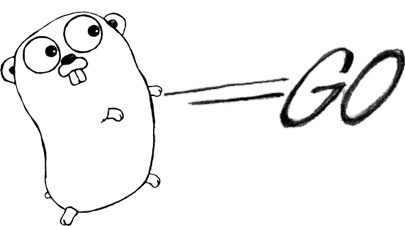
\includegraphics[width=10cm]{img/google-go-logo.jpg}
		\caption{Logo du langage de Google, Golang}
		\label{golang}
	\end{center}
\end{figure}

Le projet de communication M2M \textit{paho}\footnote{\url{http://www.eclipse.org/paho/}} fournit une librairie client Go qui est très simple d'utilisation. Un exemple est d'ailleurs donné sur la page \url{https://eclipse.org/paho/clients/golang/} et c'est lui qui a servi de base pour la mini-app. \\

Voici d'ailleurs ce que l'application fait :
\begin{figure}[H]
	\begin{center}
		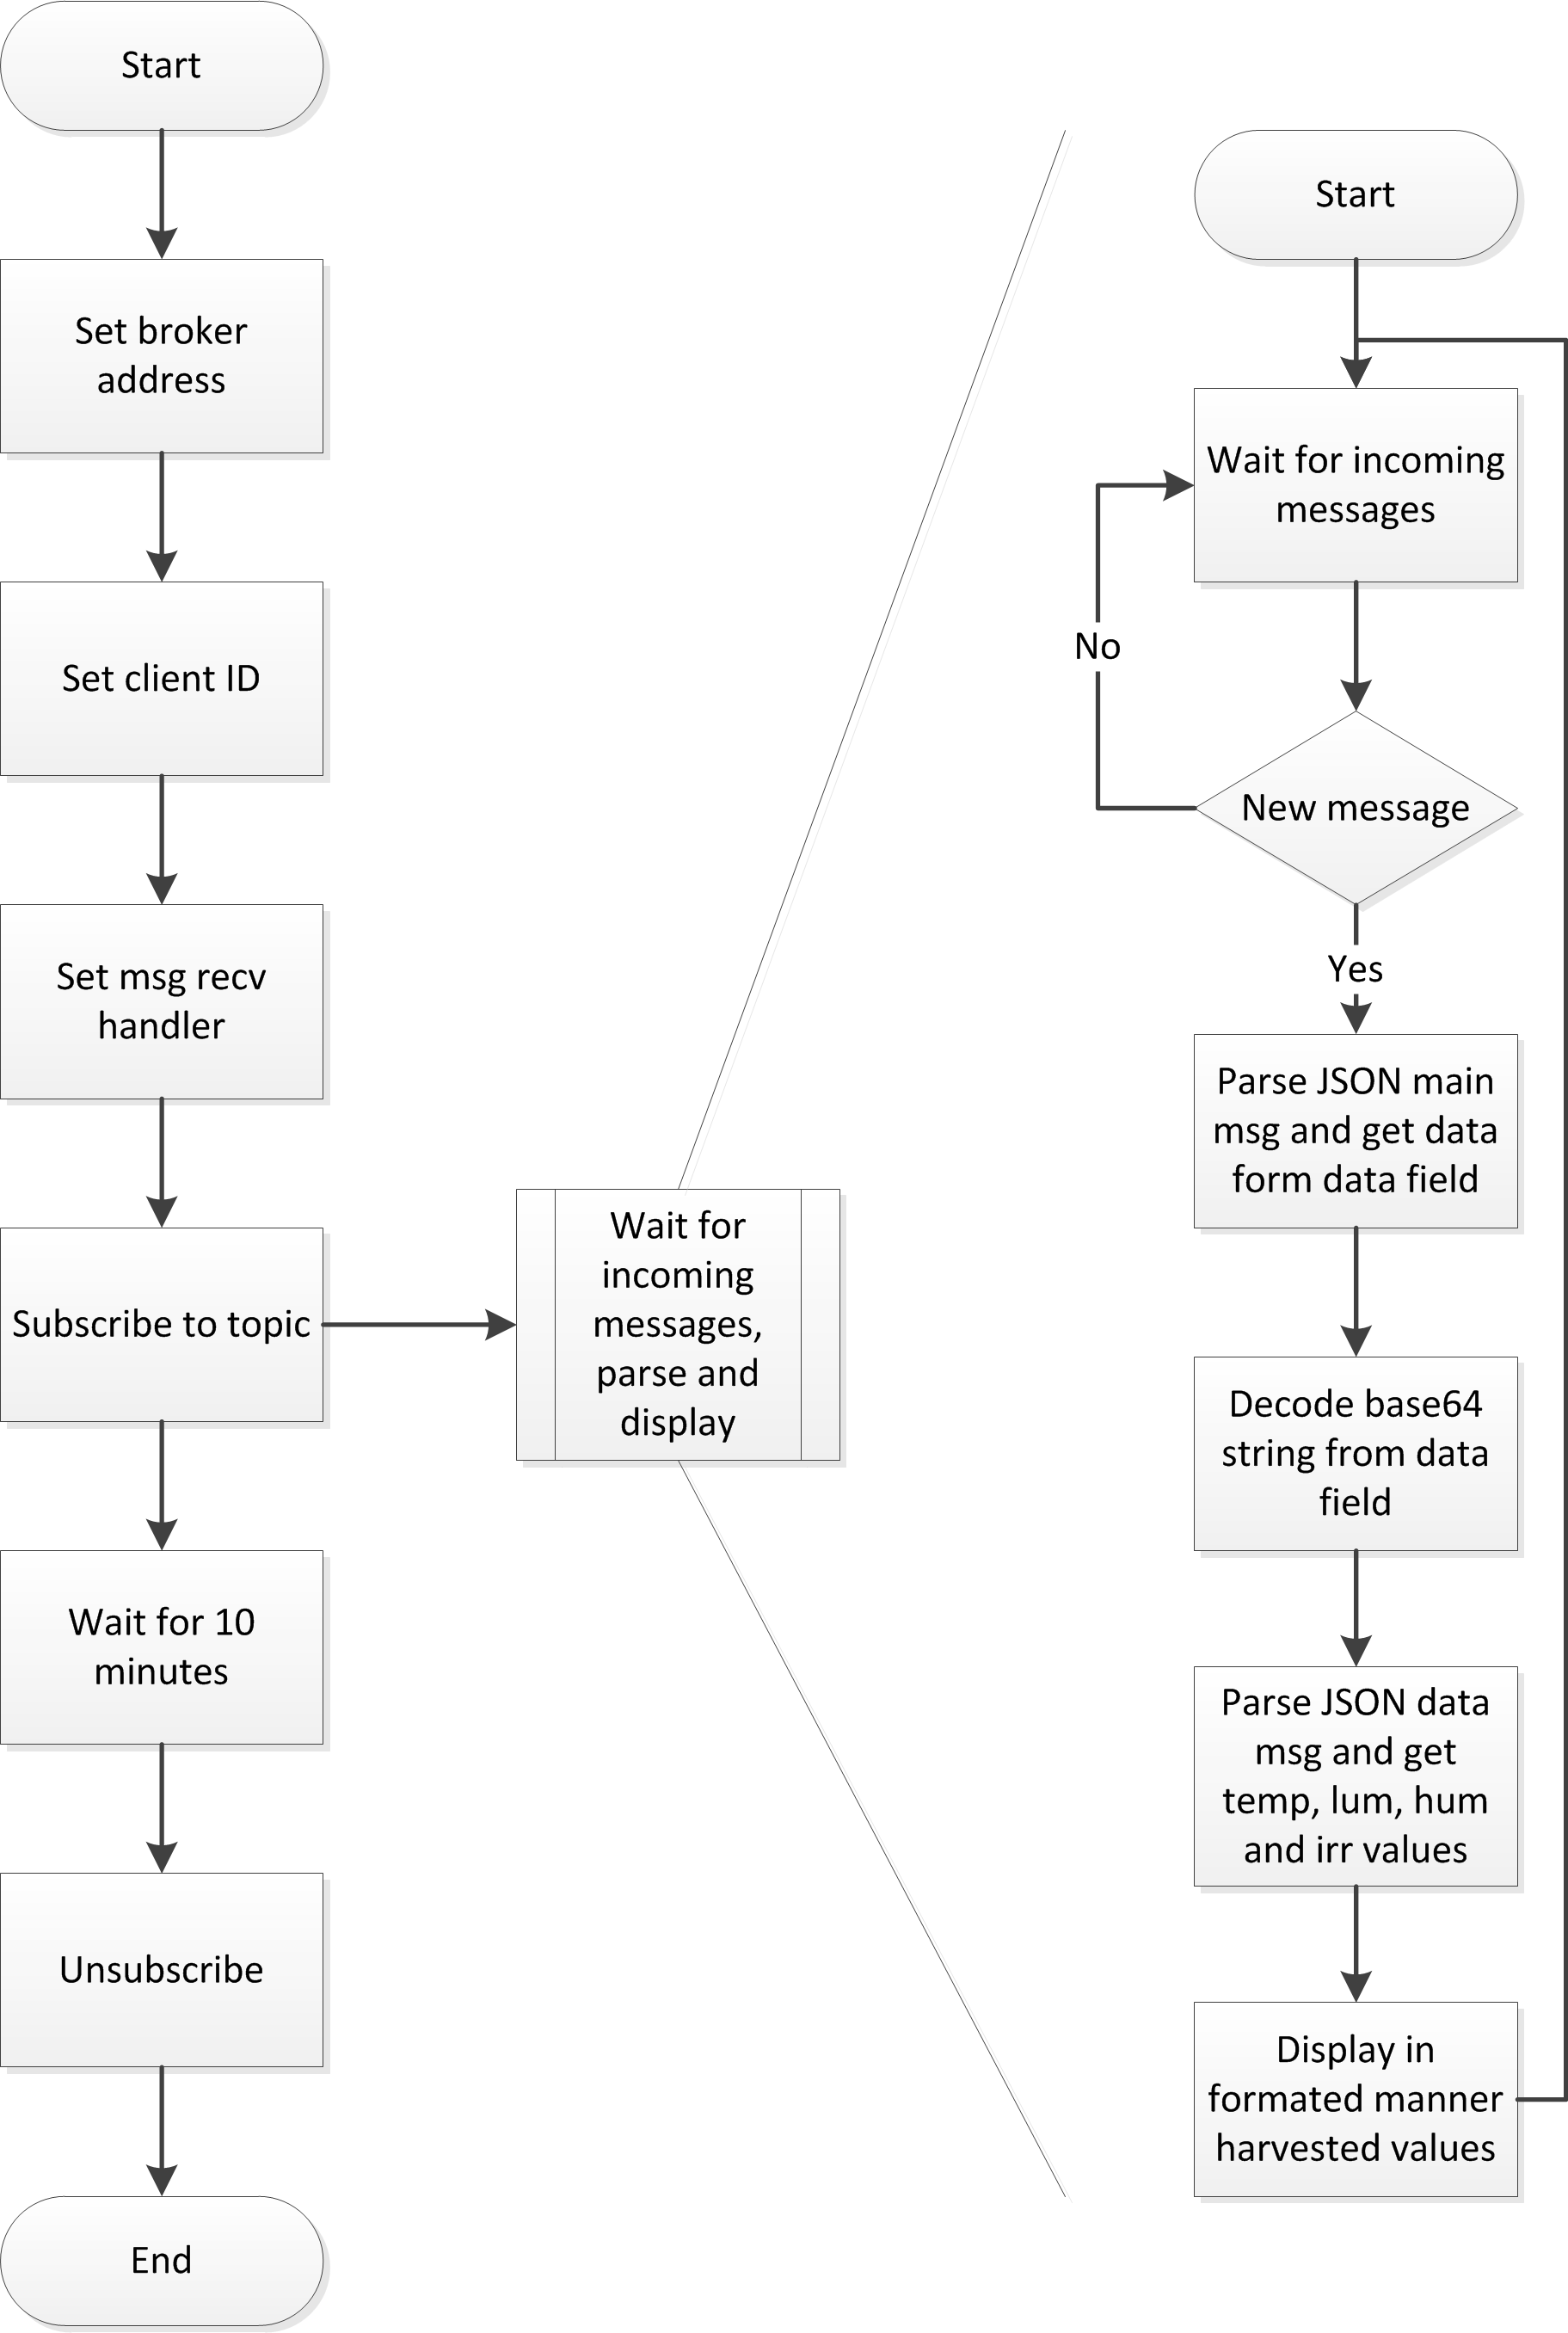
\includegraphics[width=12cm]{img/agro_app_flowchart.png}
		\caption{Étapes réalisées par l'application}
		\label{app_work_flow}
	\end{center}
\end{figure}

Les différents champs requis par le client sont remplis. Et on inscrit un callback sous forme de fonction anonyme comme récepteur des messages produits par le \textit{broker}. Dès qu'on a souscrit au bon \textit{topic}, le handler est lancé est s'exécute dès qu'un message arrive. Pendant ce temps, le programme principale attend, ici une période de 10 minutes, avant de se désinscrire du \textit{topic}. Le programme principal s'arrête et stoppe le thread de réception des messages.\\

La fonction de réception n'est appelée qu'en cas de réception. Elle ne fait pas de polling elle-même sur l'arrivée de messages. Elle même reçoit en paramètre un message encodé en JSON. On parse ce JSON pour en récupérer les données, elles-mêmes encodées en base64. Go dispose, dans sa librairie standard, de tout ce qu'il faut pour décoder ces formats. Une fois le base64 décodé en string, on décode à nouveau un JSON, qui a cette fois servi à transporter les données importantes pour notre application, la température, la luminosité, l'humidité et s'il y a lieu de s'inquiéter à propos de l'irrigation des cultures. \\

On récupère ces données et on les affiche simplement dans la console.
\begin{figure}[H]
	\begin{center}
		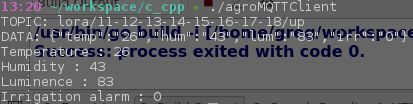
\includegraphics[width=12cm]{img/app_output.png}
		\caption{Réception et affichage d'un message}
		\label{app_output}
	\end{center}
\end{figure}